\chapter{Fundamentação Teórica} \label{cap:fundamentacao}

Nesta seção encontra-se a fundamentação teórica dos conceitos necessários ao entendimento deste trabalho de conclusão de curso. Inicialmente, será apresentada a estação meteorológica automática da EST, a principal fonte dos dados da plataforma a ser desenvolvida. Posteriormente, ainda considerando a contextualização da problemática, serão apresentados os boletins meteorológicos produzidos pelo LabInstru. Considerando o domínio da Meteorologia, dois conceitos que estarão presentes na solução proposta são apresentados: o índice de calor e a escala de Beaufort. Por fim, serão apresentados os conceitos fundamentais do processo de desenvolvimento \emph{Agile Unified Process} e do \emph{framework} web Web2py.

\section{Estação Meteorológica Automática da EST}
Uma estação meteorológica é um equipamento, assemelhado a uma torre, que possui diversos tipos de instrumentos necessários aos estudos do tempo e do clima. A leitura desses instrumentos permite conhecer o estado presente da atmosfera. Estas estações podem ser de dois tipos: convencionais e automáticas. O primeiro tipo de estação necessita da ação humana para completar seu processo de aferição e coleta dos dados. Já o segundo tipo de estação, as estações meteorológicas automáticas, não depende de uma pessoa para a realização de suas funções \cite{Vianello:Livro}.

Uma estação meteorológica automática é uma torre de observação, constituida por um conjunto de sensores eletrônicos automáticos de alta precisão, instalada no interior de um cercado, rigorosamente construída e operando segundo padrões internacionais. Inicialmente as estações automatáticas tinham como objetivo principal complementar a rede básica de estações convencionais, cobrindo regiões de difícil acesso, suprindo a falta de pessoal especializado para complementar o proceso de medições. Porém, considerando a possiblidade de observações em diferentes horários e o alto grau de confiabilidade dos dados obtidos, estas têm substituído significativamente as estações convencionais  \cite{Vianello:Livro}.

Dentre diversas outras atividades, o LabInstru administra uma estação meteorológica automática localizada nas dependências da Escola Superior de Tecnologia, ilustrada na Figura \ref{fig:ema}. Esta encontra-se em um cercado construído conforme as normas da Organização Meteorológica Mundial, com dimensões de $10 \times 15$ metros quadrados, com alambrado de $1,5$ metros pintado na cor branca. No centro deste cercado encontra-se um tripé de Campbell com $3$ metros de altura, o qual serve de suporte para diversos sensores instalados ao longo de sua extensão, bem como para os sistemas de aquisição e armazenamento dos dados, alimentação, e transmissão dos dados \cite{Labinstru:EST}.

\newpage

\begin{figure}
\begin{minipage}{\textwidth}
  \begin{minipage}[b]{0.59\textwidth}
    \centering
    	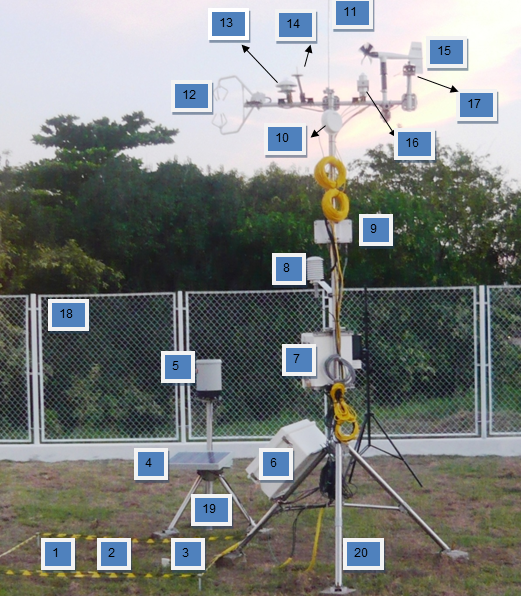
\includegraphics[width=\textwidth]{./img/ema5.png}
  \end{minipage}
  \hfill
  \begin{minipage}[b]{0.39\textwidth}
    \centering
		\begin{footnotesize}
		\begin{tabular}{cc}
		\toprule
		Item & Descrição\\
		\midrule
		1 & Reflectômetro \\
		2 & Placa de fluxo de calor no solo\\
		3 & Perfilador de temperatura no solo\\
		4 & Painel solar\\
		5 & Pluviômetro \\
		6 & Ver Figura \ref{fig:ema2}\\
		7 & Ver Figura \ref{fig:ema3}\\
		8 & Termohigrômetro\\
		9 & Caixa do sônico\\
		10 & Antena de transmissão de dados\\
		11 & Para-raio\\
		12 & Anemômetro sônico\\
		13 & Albedômetro \\
		14 & Saldo radiômetro (NR-LITE)\\
		15 & Anemômetro\\
		16 & Saldo radiômetro (CNR1)\\
		17 & Radiômetro\\
		18 & Cercado \\
		19 & Tripé de 1 metro \\
		20 & Tripé de 3 metros\\
		\bottomrule
		\end{tabular}
	\end{footnotesize}
    \end{minipage}
  \end{minipage}
	\caption{Estação meteorológica automática da EST e descrição dos seus componentes. Fonte: \cite{Labinstru:EST}.}\label{fig:ema}
\end{figure}

Próximo ao tripé da haste, encontram-se instalados os sensores para monitoramento das condições do solo. São eles:
\begin{enumerate}
	\item Reflectômetro para medida de conteúdo de água no solo (CS 616 - Campbell);
	\item Placa de fluxo de calor no solo (HFP01 - Hukseflux) instaladas em 5cm;
	\item Perfilador de temperatura no solo (STP01 - Hukseflux) medindo a temperatura nas profundidades de 2, 5,   10, 20 e 50 cm;
\end{enumerate}

Ao longo da haste do tripé encontram-se os seguintes sensores:
\begin{enumerate}
	\item Anemômetro sônico (CSAT3 - Campbell) para gerar medidas das componentes ortogonais do vento e temperatura virtual do ar;
	\item Anemômetro (05106 - Young) para medida da direção e velocidade do vento;
	\item Barômetro (CS106 - Vaisala) para medir a pressão atmosférica;
	\item Termohigrômetro (HMP45C - Vaisala) para medir temperatura e umidade do ar;
	\item Saldo radiômetro (NR-LITE – Kipp \& Zonen) para a medida do saldo de radiação;
	\item Saldo radiômetro (CNR1 - Kipp \& Zonen) para medidas da radiação solar incidente e refletida, e radiação terrestre e atmosférica emitidas;
	\item Radiômetro PAR (PAR LITE - Kipp \& Zonen) para a medida da componente fotossinteticamente ativa da radiação solar;
	\item Albedômetro (CMA11 - Kipp \& Zonnen) para medidas das radiações solar incidente e refletida \cite{Labinstru:EST}.
\end{enumerate}

Ao lado do tripé de $3$m, um segundo tripé de $1$ metro de altura serve de suporte para um pluviômetro (TB4 - Hydrological Services), que totaliza a precipitação, e para o painel solar. Há também a caixa do sônico, a antena de transmissão dos dados e um pára-raios. Uma caixa de poliéster reforçada com fibra de vidro, abriga o sistema de aquisição dos dados (\emph{datalogger}), barômetro e interface para gravação dos dados (NL 115, Campbell) \cite{Labinstru:EST}, conforme ilustrado detalhadamente na Figura \ref{fig:ema2}. Uma outra caixa abriga duas baterias, o controlador de carga e um roteador, conforme mostra a Figura \ref{fig:ema3}.

\begin{figure}[h!]
	\centering
	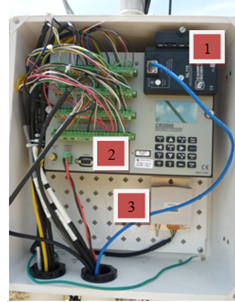
\includegraphics[width=0.3\textwidth]{./img/ema6.png}
	\caption{Detalhamento do item 6 da Figura \ref{fig:ema}. O item 1 indica a interface para gravação dos dados, o item 2 indica o \emph{datalogger} e o item 3 indica o barômetro. Fonte: \cite{Labinstru:EST}} \label{fig:ema2}
\end{figure}

\begin{figure}[h!]
	\centering
	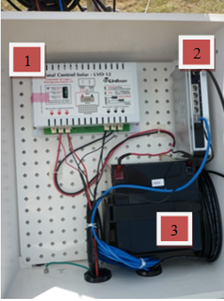
\includegraphics[width=0.3\textwidth]{./img/ema7.png}
	\caption{Detalhamento do item 7 da Figura  \ref{fig:ema}, referente à transmissão de dados. O item 1 consiste em um regulador de voltagem, o item 2 em um roteador e o item 3 em uma bateria. Fonte: \cite{Labinstru:EST}} \label{fig:ema3}
\end{figure}

Todos os sinais dos sensores, bem como a voltagem da bateria, são medidos por um sistema de aquisição e armazenamento de dados (\emph{datalogger}), programado para realizar leitura a cada segundo e gravar os dados em um certo intervalo de tempo. A transmissão dos dados pode ser realizada de duas formas: por meio da gravação dos dados em um cartão removível de $2$ GB ou via conexão wireless utilizando o protocolo TCP/IP entre o \emph{datalogger} CR3000 e um computador remoto, contendo um programa específico para a correta transmissão do dados. A Figura \ref{fig:ema4} exemplifica o passo a passo da transmissão.

\begin{figure}[H]
	\centering
	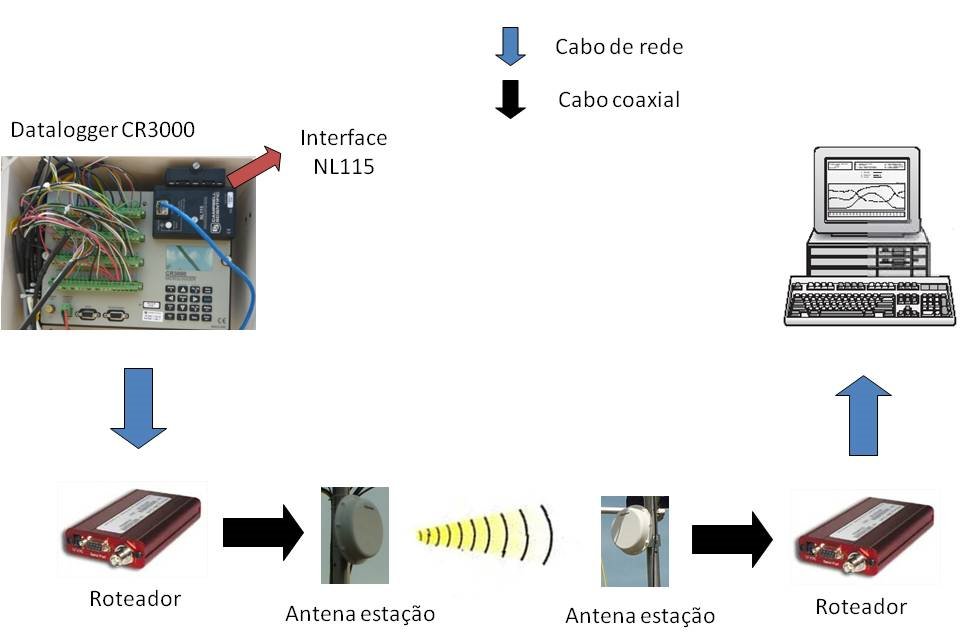
\includegraphics[width=1\textwidth]{./img/ema4.png}
	\caption{Esquema de transmissão dos dados da estação meteorológica. Fonte: \cite{Labinstru:EST}} \label{fig:ema4}
\end{figure}

Após a transmissão, a equipe do LabInstru passa a ter acesso aos dados capturados pela estação.  Além das informações meteorológicas, a estação também fornece dados de controle, tais como carga da bateria, tempo estimado de funcionamento, etc. Todos os dados produzidos são persistidos em um arquivo-texto de maneira serializada a intervalos de tempo fixos e pré-determinados de dez minutos. O arquivo, embora possua uma estrutura textual, assemelha-se a uma ``tabela'' como maneira de organizar os dados. A Figura \ref{fig:exemploBaixa1} ilustra um trecho deste arquivo. As linhas 1-8 mostram o cabeçalho do arquivo, que descreve quais variáveis serão persistidas a partir deste momento pela estação meteorológica. As linhas 9-11 e 12-14 exemplificam dois registros de dados da estação meteorológica feitos no dia $05$ de Fevereiro de $2014$ às 09h40min e às 09h50min, respectivamente.

Atualmente, os responsáveis pelo LabInstru abrem este arquivo de maneira manual e, utilizando softwares editores de texto e de planilhas, geram sumários, estatíticas, gráficos, dentre outros. Como pode ser visto, explorar manualmente estes arquivos, especialmente considerando um longo período de tempo, é um trabalho difícil e demorado. A minimização destas dificuldades é uma das motivações para a realização deste trabalho.

\begin{figure}[H]
\centering
\begin{scriptsize}
\fbox{
    \begin{minipage}{1\textwidth}
	    \internallinenumbers
	    `TIMESTAMP', `RECORD', `batt\_volt\_Min', `PTemp', `NRLite\_Avg', `CM3Up\_Avg', `CM3Dn\_Avg', `CG3UpCorr\_Avg', `CG3DnCorr\_Avg', `CNR1TC\_Avg', `CMA11Up\_Avg', `CMA11Dn\_Avg', `LI190S\_Avg', `VW\_Avg', `HFP01\_Avg', `STP01\_50cm\_Avg', `STP01\_20cm\_Avg',  `STP01\_10cm\_Avg', `STP01\_5cm\_Avg', `STP01\_2cm\_Avg', `CS106\_Avg', `HMP45C\_Temp\_Avg', `HMP45C\_RH\_Avg', `WindSpeed', `WindDirection', `TB4\_Tot', `TS', `RN', `', `', `W/m2', `W/m2', `W/m2', `W/m2', `W/m2', `deg\_C', `W/m2', `W/m2', `umol/mol', `\%', `W/m2', `deg\_C', `deg\_C', `deg\_C', `deg\_C', `deg\_C', `hPa', `dec\_C', `\%', `m/s', `Deg', `mm', `', `', `Min', `Smp', `Avg', `Avg', `Avg', `Avg', `Avg', `Avg', `Avg', `Avg', `Avg', `Avg', `Avg', `Avg', `Avg', `Avg', `Avg', `Avg', `Avg', `Avg', `Avg', `WVc:Averaged\_Value', `WVc:Averaged\_Value', `Tot'\\
`2014-02-05 09:40:00',  118726,  13.23,  28.78, 233.1908, 359.7406, 60.10703, 1249.177, 1290.342, 115.3246, 363.9763, 65.63671, 448.9503, 0.2546729, `NAN',  29.45563, 28.85126, 28.97074, 29.36523, 29.92229, 1009.477, 27.5499, 79.00884, 0.7635838, 103.2079, 0\\
`2014-02-05 09:50:00',  118727, 13.24, 29.03, 218.5598, 342.636, 56.87075, 1259.051, 1300.909, 116.1448, 346.5667, 62.29135, 430.326, 0.2546285, `NAN',  29.45018, 28.87249, 29.0521, 29.47018, 29.96688, 1009.529, 27.53578, 78.62649, 0.8266301, 113.4006, 0
    \end{minipage}
}
\end{scriptsize}
\caption{Exemplo de um trecho dos dados encontrados no arquivo produzido pela estação meteorológica.} \label{fig:exemploBaixa1}
\end{figure}

\newpage

\section{Boletim Meteorológico do LabInstru} \label{sec:boletim}
O \emph{boletim meteorológico diário} do LabInstru é um informativo dos dados registrados pela estação meteorológica da EST/UEA através da utilização de imagens ilustrativas, visando apresentar diferentes aspectos do tempo, tais como: temperatura máxima e mínima, ocorrência ou não de precipitação, velocidade máxima do vento, rajada e índice de calor. Estes boletins são produzidos para divulgação junto à comunidade, como uma maneira resumida de apresentar dados relacionados às variáveis meteorológicas registradas na estação. Exemplos desses boletins meteorológicos produzidos pelo LabInstru podem ser visualizados na Figura \ref{fig:bm}.

\begin{figure}[h!]
	\centering
	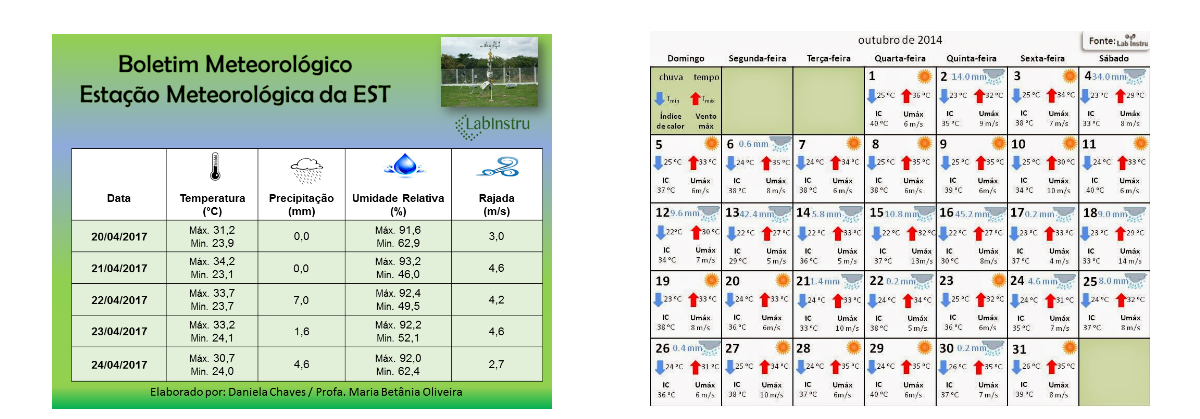
\includegraphics[width=0.9\textwidth]{./img/bm.png}
	\caption{Exemplos de boletins meteorológicos produzidos pelo LabInstru. Fonte: \cite{Labinstru:EST}} \label{fig:bm}
\end{figure}

A produção de boletins meteorológicos é uma das atribuições do LabInstru e pode ser visto como uma forma de fácil assimilação dos dados meteorológicos produzidos pela equipe do laboratório. Considerando a sua importância, um trabalho anterior visou produzir estes boletins de maneira automática através de uma ferramenta intitulada BoCliMa, acrônimo para Boletim Climático de Manaus \cite{Lima:Artigo}.

O BoCliMa produz boletins meteorológicos a partir dos dados da estação meteorológica da EST/UEA, exibindo boletins por turno e diários. Cada boletim contempla a data, ocorrência ou não de precipitação, temperaturas máxima e mínima, índice de calor e rajada de vento, que se caracteriza como a maior velocidade do vento registrada em um dia. Um exemplo de boletim produzido pelo BoCliMa encontra-se ilustrado na Figura \ref{fig:boclima}.

\begin{figure}[h!]
	\centering
	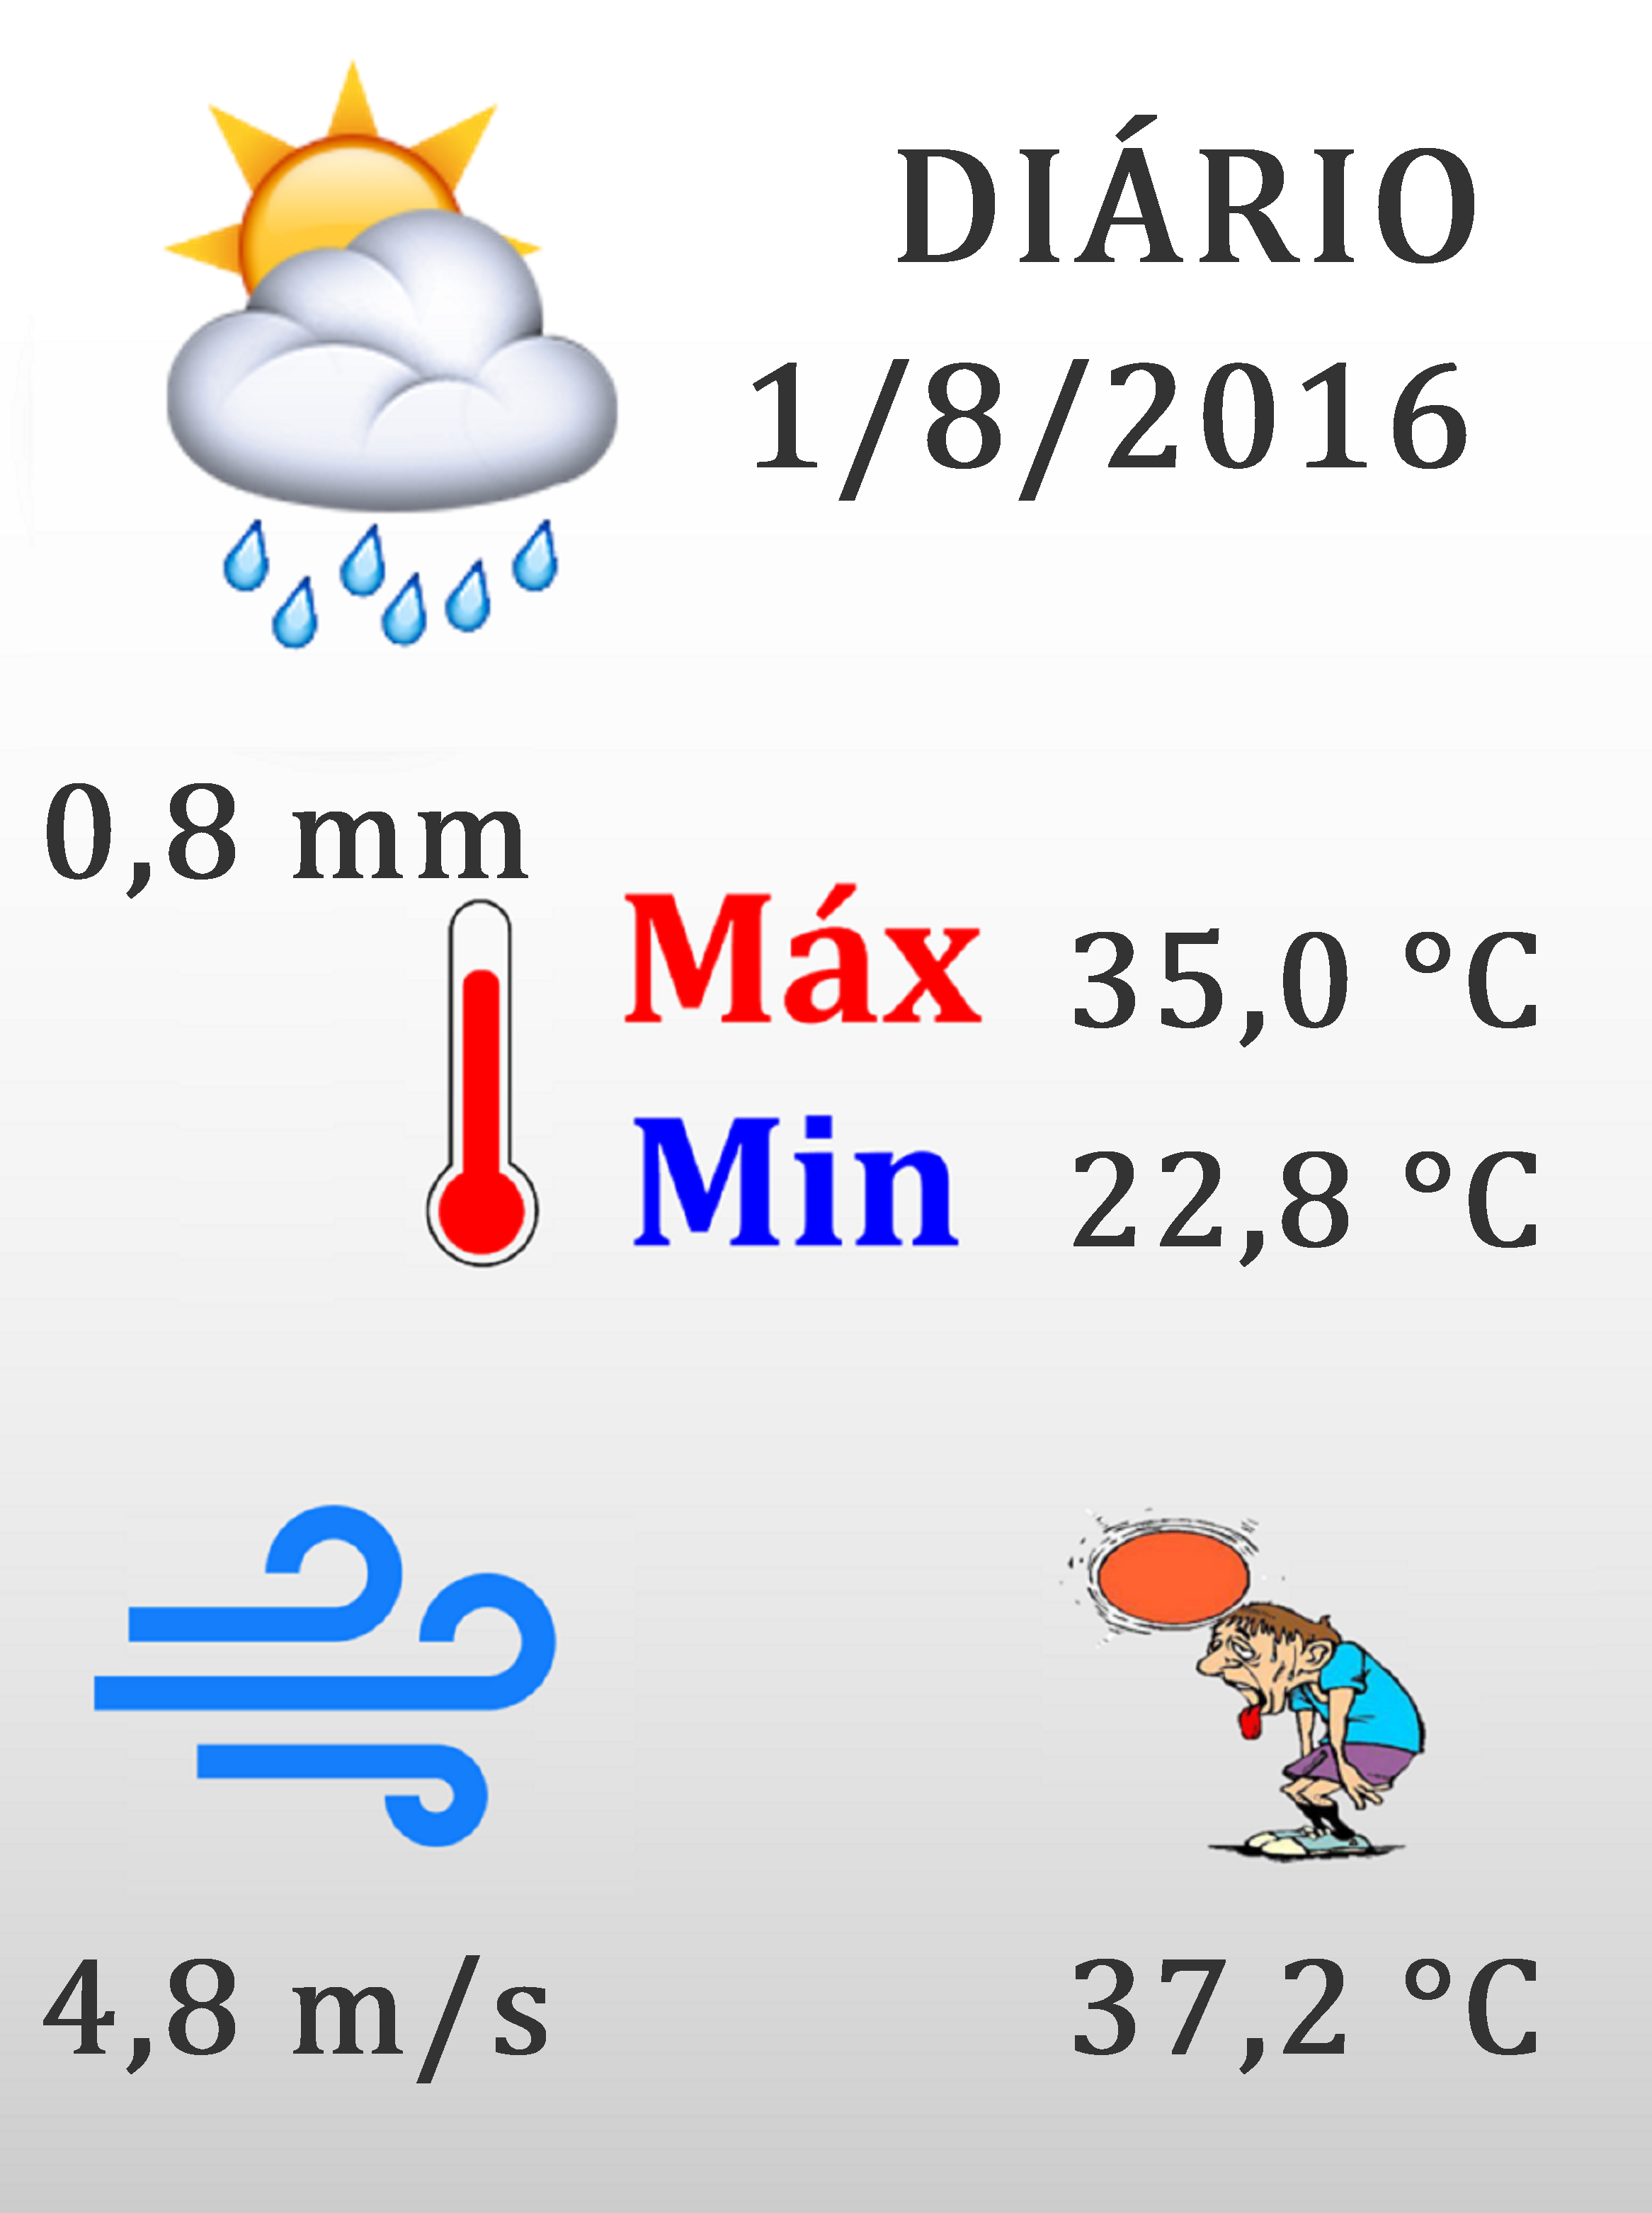
\includegraphics[width=0.3\textwidth]{./img/boclima}
	\caption{Exemplos de boletim meteorológico gerado pelo BoCliMa. } \label{fig:boclima}
\end{figure}

A produção de um boletim meteorológico pelo BoCliMa demanda que o usuário forneça os arquivos com as medições do dia que deseja produzir o boletim. Para tanto, o usuário precisa manualmente consultar os diferentes arquivos produzidos pelas estações e sintetizar um novo arquivo que possa alimentar o BoCliMa. Além destas dificuldades, é possível também observar que no boletim meteorológico produzido, não há uma legenda adequada das informações disponibilizadas (indicando, por exemplo, o índice de calor, as rajadas, etc.) e que também não possui referências ao LabInstru e nem tampouco à cidade de Manaus.

Minimizar as limitações identificadas no boletim produzido pelo BoCliMa e tirar proveito da facilidade de integrar a produção de boletins a uma plataforma que já contempla as medições da estação meteorológica da EST são aspectos que foram considerados no escopo deste trabalho de conclusão de curso, visando prover um melhor suporte na realização das atividades do LabInstru.


\section{Índice de Calor}
O \emph{índice de calor} é uma temperatura aparente que representa a percepção da pele humana para as condições de temperatura e umidade aos quais está submetida, estando a pessoa sob sombra e submetida a ventos fracos \cite{Steadman:IndiceCalor}.É um dado meteorológico derivado a partir da temperatura máxima e da umidade relativa do ar obtida no instante da temperatura máxima, combinados por meio de uma análise de regressão múltipla, conforme proposto por Rothfusz \cite{Rothfusz:HeatIndex}. O cálculo do índice de calor é obtido como segue:

\begin{eqnarray}
Index_{heat} &=& - 42,379 + (2,04901523 \times T) + (10,14333127 \times rh) - (0,22475541 \times T \times rh) \nonumber\\
& \ &  - (6,83783 \times 10^{-3}\times T^2) - (5,481717 \times 10^2 \times rh^2) + (1,22874 \times 10^{-3} \times T^2 \times rh)  \nonumber\\
& \ &  + (8,5282 \times 10^{-4} \times T \times rh^2) - (1,99 \times 10^{-6} \times T^2 \times rh^2),
\end{eqnarray} em que $T$ é a temperatura máxima do dia em graus Fahrenheit e $rh$ é a umidade relativa do ar em \% no instante da temperatura máxima.

Há dois tipos de ajustes necessários no cálculo do índice de calor. Se $rh < 13\%$ e a temperatura encontra-se entre $26,7 ^{\circ}C$ e $44,4 ^{\circ}C$, é necessário subtrair do $Index_{heat}$ o seguinte valor de ajuste:

\begin{equation}
\textrm{ADJUSTEMENT 1} = [(13-rh)/4] \times \sqrt{\frac{17 - abs(T - 95)}{17}},
\end{equation} em que $abs$ denota o valor absoluto. O outro tipo de ajuste ocorre se $rh > 85\%$ e $T$ encontra-se entre $26,7 ^{\circ}C$ e $30,6 ^{\circ}C$. Neste caso, é necessário subtrair do $Index_{heat}$ o valor de ajuste:

\begin{equation}
\textrm{ADJUSTEMENT 2} = [(rh - 85)/10]\times(87-T)/5].
\end{equation} 

Assim, para cada dia de observação de dados meteorológicos, é importante obter o índice de calor. Sendo possível a partir desse valor, utilizando uma tabela específica, classificar o índice de calor de acordo com seu nível de alerta e saber as consequências que o mesmo pode trazer para saúde do homem, vide Tabela \ref{tab:indiceCalor}. Este dado auxilia na tomada de decisão para evitar problemas de saúde pelo excesso de exposição ao calor, tais como cãimbras, esgotamento, dentre outros, que até podem culminar em óbito \cite{Silva:CalorTrabalho,Lima:Artigo}.

\begin{table}[h!]
  \caption{Níveis de alerta e suas consequências à saúde humana. Fonte: Adaptado de National Weather Service, Weather Forecast Office, NOAA} \label{tab:indiceCalor}
  \centering
\begin{tabular}{ccp{7cm}}
 \toprule
 \textbf{Nível de Alerta} & \textbf{Índice de Calor} & \textbf{Sintomas}\\
 \midrule
Perigo Extremo & 54 $^{\circ}C$ ou mais & Insolação; risco de acidente vascular cerebral (AVC) iminente.\\
Perigo & 41,1 $^{\circ}C$ - 54 $^{\circ}C$  & Câimbras, insolação, esgotamento físico. Possibilidade de danos cerebrais (AVC) para exposições prolongadas com atividades físicas.\\
Cautela Extrema & 32,1 $^{\circ}C$ - 41 $^{\circ}C$ & Possibilidade de câimbras, de esgotamento físico e insolação para exposições prolongadas e atividades físicas.\\
Cautela & 27,1 $^{\circ}C$ - 32 $^{\circ}C$ & Possível fadiga em casos de exposições prolongadas e práticas de atividades físicas.\\
Não há alerta & IC < 27 $^{\circ}C$ & Não há problemas\\
\bottomrule
\end{tabular}
\end{table}

\section{Escala de Beaufort}
A Escala de Beaufort é uma tabela criada pelo meteorologista anglo-irlandês Francis Beaufort no inicio do Século XIX que tem como objetivo classificar a intensidade dos ventos, tendo como parâmetros a velocidade dos ventos e os efeitos resultantes das ventanias no mar e em terra. Segundo a Escala de Beaufort, por exemplo, ventos na escala 8 são capazes de mover as folhas das árvores e inicializar os trabalhos de moinhos (efeitos em terra), no mar, resulta uma ligeira ondulação sem rebentação (aspecto do mar) \cite{MetOffice:Beaufort}. Em 2007, a escala de Beaufort passou por uma adaptação para níveis continentais \cite{Sentelhas:EscalaBeaufort}, cujo resultado é ilustrado na  Tabela \ref{tab:beaufort}.

\begin{table}[h!]


  \caption{Escala de Beaufort. Fonte: \cite{Sentelhas:EscalaBeaufort}} \label{tab:beaufort}
  \centering
\begin{tabular}{ccc}
 \toprule
 \textbf{Escala} & \textbf{Classificação} & \textbf{Velocidade (m/s)}\\
 \midrule
0 & Calmo & $<$ 0,5\\
1 & Quase calmo & 0,5 a 1,5\\
2 & Brisa amena & 1,6 a 2,9\\
3 & Vento Leve & 3,0 a 5,7\\
4 & Vento Moderado & 5,8 a 8,3\\
5 & Vento Forte & 8,4 a 11,1\\
6 & Vento Muito Forte &  11,2 a 13,9\\
7 & Vento fortíssimo & 14,0 a 16,6\\
8 & Ventania & 16,7 a 20,9\\
9 & Vendaval & 21,0 a 27,8\\
10 & Tornado, furacão & $>$ 27,8\\
\bottomrule
\end{tabular}
\end{table}

Saber especificar a escala de uma determinada medição para a velocidade do vento utilizando a escala de Beaufort e consultar os efeitos que esse tipo de vento pode ocasionar sobre o ambiente em que ocorreu são informações comumente divulgadas em boletins meteorológicos para a população em geral, sendo úteis, inclusive, na emissão de alertas sobre  ventanias fortes, tempestades e até mesmo furacões.


\section{Processo Unificado Ágil}
Em contextos nos quais há uma demanda por software que precisa ser rapidamente atendida ou quando os requisitos mudam rapidamente, processos de desenvolvimento ágil são recomendados. Estes processos possuem natureza iterativa, nos quais as fases de especificação, projeto, desenvolvimento e teste se intercalam. Como consequência, o software é entregue não em uma versão final acabada, mas em uma série de incrementos de novas funcionalidades.
\cite{Sommerville:Livro}.

Na década de 1990, houve uma demanda ainda maior para que os esforços das equipes de desenvolvimento se concentrassem no software somente, diminuindo o ônus em projeto e documentação. Em resposta, foi proposto o  ``Manifesto para o Desenvolvimento Ágil'' (\textit{The Manifesto for Agile Software Development}) \cite{KentBeck:ManifestoAgil}, no qual foi proposta a abordagem iterativa para especificação, desenvolvimento e entrega do software para cenários com requisitos que mudam rapidamente e nos quais se deseja entregar um software rapidamente ao cliente. O Manifesto para o Desenvolvimento Ágil possui quatro valores, são eles:

\begin{enumerate}
	\item Indivíduos e interações acima de processos e ferramentas;
	\item Software operacional acima de documentação completa;
	\item Colaboração dos clientes acima de negociação contratual;
	\item Respostas a mudanças acima de seguir um plano \cite{Pressman:Livro}.
\end{enumerate}

Os princípios do Manifesto Ágil consideram como prioridade a satisfação do cliente e o acolhimento dos pedidos de alterações. A medida de progresso considerada é a entrega de software em funcionamento ao cliente, razão pela qual há várias entregas do software desenvolvido em intervalos pequenos de tempo. Ressalta-se a importância da motivação da equipe engajada no projeto, que deve trabalhar em conjunto diariamente, com uma comunicação fluida e, preferencialmente, presencial. A simplicidade, auto-organização e avaliação em intervalos regulares complementam esses princípios \cite{KentBeck:ManifestoAgil}.

Atualmente, existe um vasto número de modelos de processo ágeis que satisfazem aos princípios do Manifesto Ágil, inclusive com muitas semelhanças filosóficas e práticas entre eles. Exemplos de modelos de processos ágeis são: SCRUM, \emph{eXtreme Programming}, \emph{Feature Driven Development}, \emph{Agile Unified Process}, dentre outros.

O \emph{Processo Unificado Ágil} (AUP - \textit{Agile Unified Process}), em particular, é um modelo ágil para o desenvolvimento de software. O AUP é baseado em um processo de desenvolvimento de software clássico, o RUP (\textit{Rational Unified Process}). O RUP é destinado a grandes projetos que envolvam um grande número de pessoas em sua equipe de desenvolvimento. Ao conceber o AUP, o seu criador, Scott Ambler, procurou adaptar as boas práticas do RUP a pequenos projetos. Através de uma metodologia simples e de fácil compreensão, usando técnicas e conceitos ágeis para o desenvolvimento de software, o AUP segue uma filosofia ágil permanecendo fiel às práticas do RUP \cite{Ambler:Livro}.


O AUP possui quatro fases de desenvolvimento, são elas:

\begin{itemize}
	\item \textbf{Concepção (\textit{Inception}).} O objetivo é identificar o escopo inicial do projeto e a arquitetura potencial do sistema a fim de gerar estimativas financeiras e prover informações que subsidiem a aceitação pelas partes interessadas;
	\item \textbf{Elaboração (\textit{Elaboration}).} O objetivo é prover uma arquitetura central, resolução dos altos riscos e definição de estimativas mais realistas;
	\item \textbf{Construção (\textit{Construction}).} O objetivo é construir o software, trabalhando em uma base incremental regular, que atende às necessidades de maior prioridade das partes interessadas no projeto;
	\item \textbf{Transição (\textit{Transition}).} O objetivo é validar e implantar o sistema em seu ambiente de produção.
\end{itemize}

As fases do AUP não são realizadas em cascata. Ao contrário, há diversas iterações e podem existir atividades de fases distintas sendo executadas em paralelo. Uma ideia do ciclo de vida do AUP que ilustra esta característica pode ser visualizada na Figura \ref{fig:aupciclo}.

\begin{figure}[H]
	\centering
	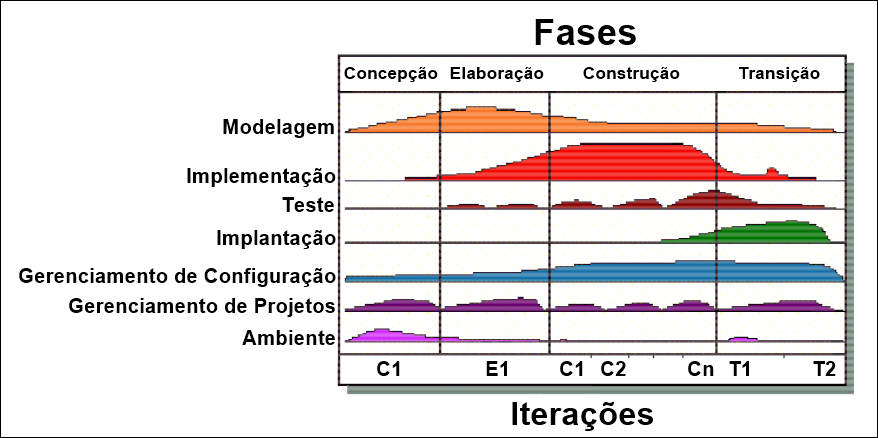
\includegraphics[scale=0.7]{./img/aupOficial.png}
	\caption{Ciclo de vida do AUP.} \label{fig:aupciclo}
\end{figure}

Ainda conforme a Figura \ref{fig:aupciclo}, é possível identificar as sete disciplinas que compõem o AUP. Elas definem um conjunto de atividades (e artefatos relacionados) que são realizados ao longo das iterações de desenvolvimento. Estas disciplinas são definidas como segue:

\begin{itemize}
	\item \textbf{Modelagem (\textit{Model})}. O objetivo desta disciplina é promover o entendimento do negócio da organização, o domínio do problema a ser abordado pelo projeto, e a identificação de uma solução viável para resolver o domínio do problema;
	\item \textbf{Implementação (\textit{Implementation})}. O objetivo desta disciplina é o de transformar o(s) modelo(s) em código executável e executar um nível básico de testes, nomeadamente os testes de unidades;
	\item \textbf{Teste (\textit{Test})}. O objetivo desta disciplina é a realização de uma avaliação objetiva para garantir a qualidade. Isto inclui as atividades de validação e verificação dos requisitos;
	\item \textbf{Implantação (Deployment)}. O objetivo desta disciplina é planejar a entrega do sistema e executar este plano a fim de tornar o sistema disponível para os usuários finais;
	\item \textbf{Gerenciamento de Configuração (\textit{Configuration Management})}. O objetivo desta disciplina é o de gerir o acesso aos artefatos criados durante todas as fases do desenvolvimento do software. Isso inclui não apenas controlar versões de artefatos ao longo do tempo, mas também controlar e gerenciar mudanças;
	\item \textbf{Gerenciamento de Projetos (\textit{Project Management})}. O objetivo desta disciplina é a de dirigir as atividades que ocorrem no projeto. Isto incluir a gestão de riscos, a coordenação de pessoas e controle de prazos e orçamento;
	\item \textbf{Ambiente (\textit{Environment})}. O objetivo desta disciplina é o de apoiar o resto do esforço, garantido que o processo adequado, orientação (normas e diretrizes) e ferramentas (hardware, software, etc) estejam disponíveis para a equipe quando necessário \cite{Ambler:Livro}.
\end{itemize}

Durante uma iteração, o trabalho prossegue na maioria ou em todas as disciplinas. Entretanto, o esforço relativo no decorrer destas disciplinas muda ao longo do tempo. As iterações iniciais tendem a dar uma ênfase maior aos requisitos e ao projeto, enquanto que as últimas disciplinas dão a esses itens uma ênfase menor, à medida que os requisitos e o projeto central se estabilizam por meio de um processo de realimentação e adaptação \cite{Larman:Livro}.


\section{\emph{Framework} Web2py} \label{sec:web2py}
Web2py é um \emph{framework open source}, criado por Massimo Di Pierro, escrito e programável em Python, que possui como principal objetivo o desenvolvimento ágil de aplicações web seguras baseadas em bancos de dados \cite{Pierro:Livro}. O foco do Web2py consiste em permitir que o desenvolvedor concentre-se apenas na aplicação que está desenvolvendo, considerando o provimento de três pilares, que são a simplicidade, o desenvolvimento veloz e a segurança \cite{Duarte:Web2py}.

Por simplicidade no contexto do Web2py, prentende-se reduzir a curva de aprendizagem e tempo para desenvolvimento e/ou manutenção. Por isso, o Web2py é considerado um framework \textit{full-stack} sem dependências, ou seja, ele não necessita de instalação e configuração de arquivos ou outros programas. Ele já é disponibilizado de maneira pronta para o desenvolvimento e com todos os seus módulos funcionando, incluindo o servidor web (Rocket WSGI Web Server), banco de dados (por padrão SQLite) e a IDE web (acessível pelo seu navegador) que fornece acesso a todas as principais funcionalidades \cite{Pierro:Livro}.

O segundo pilar, desenvolvimento veloz, é instanciando no Web2py por meio da existência de comportamentos padrões. O programador deve sobrescrevê-los apenas se necessário. Assim, quando os modelos de dados são especificados, tem-se acesso a um painel web de administração do banco de dados, formulários automáticos, dentre outros. Há que se mencionar ainda a facilidade na exportação de dados, disponibilizados em XML, JSON, dentre outros, e também o fornecimento de \emph{wdigets} de alto nível, permitindo a construção ágil de aplicações web relativamente complexas \cite{Gordon:Web2pycookbook}.

Quando se fala em segurança, pode-se destacar a camada de abstração do banco de dados do Web2py, conhecida com DAL (\textit{Database Abstraction Layer}), que elimina a possibilidade de \textit{SQL Injection}. A linguagem para templates previne contra \textit{Cross Site Scripting}. Os formulários gerados pelo Web2py fornecem validação e bloqueiam a ameaça de \textit{Cross Site Request Forgeries}. Senhas são sempre armazenadas como \textit{hashes}.  Sessões são armazenadas por padrão apenas no servidor, afim de prevenir \textit{Cookie Tampering} e cookies de sessões possuem  identificadores únicos e próprios visando previnir roubos \cite{Pierro:Livro}.

A simplicidade e o desenvolvimento veloz podem ser consideradas as principais justificativas da adoção do framework Web2py como plataforma de desenvolvimento deste trabalho. Menciona-se também a utilização da linguagem de programação Python; a fácil aprendizagem dos conceitos relativos a este \emph{framework}, justificado pelo cronograma de desenvolvimento relativamente curto; e também aspectos de caráter mais técnico e tecnológico, como a possibilidade de integração com diferentes bancos de dados \emph{open source}, a utilização de tecnologias como Bootstrap e jQuery e o fato do Web2py seguir o padrão arquitetural MVC, que permite uma melhor organização do código.

\subsection{Padrão de Projeto MVC}

O MVC (do inglês, \emph{Model-View-Controller}) é o padrão de projeto mais popularmente adotado pelos \emph{frameworks} de desenvolvimento de aplicações web. Este padrão de projeto incentiva o desenvolvedor a separar as camadas de negócio(\emph{Model}) e de apresentação dos dados (\emph{View}), por meio da inclusão de uma camada de controle de fluxo de trabalho(\emph{Controller}), que atua como uma camada intermediária\cite{Pierro:Livro}. Uma visão geral do padrão MVC é ilustrada na Figura \ref{fig:padraomvc}.

\begin{figure}[H]
	\centering
	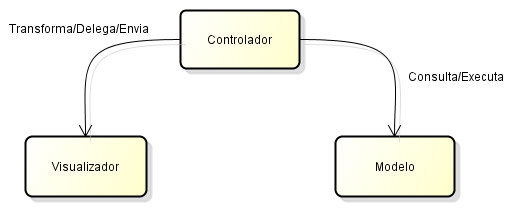
\includegraphics[width=0.6\textwidth]{./img/mvc.png}
	\caption{Visão geral do padrão de projeto MVC. Fonte: \cite{Weissman:MVC} \label{fig:padraomvc}}
\end{figure}

O \textit{modelo} diz respeito à toda a parte do sistema responsável pela lógica de negócio e seus componentes auxiliares, como persistência, criação das tabelas de banco de dados, definição das classes utilizadas na aplicação, etc. O \textit{visualizador}, por sua vez, é a parte visível ao usuário final. No caso das aplicações web, é a página HTML resultante desta camada. Por fim, o \emph{controlador} sincroniza a interação entre as duas camadas anteriores.Por exemplo, quando o usuário clica em um \textit{link} da página HTML exibida, o controlador é acionado e transforma os parâmetros de entrada (String geralmente) para um formato compatível com a camada de negócio (inteiros, doubles, objetos de classes, etc), cujo resultado do  processamento é recebido pelo controlador, que o modifica, caso necessário, e em seguida o envia à camada de visualização para que seja apresentado ao usuário final \cite{Weissman:MVC}.

O Web2py adota em seu processo de desenvolvimento o MVC como padrão de projeto, e isso pode ser facilmente percebido visualizando a estrutura de diretórios criada pelo framework, visando assim, facilitar o gerenciamento de projetos a serem desenvolvidos, proporcionando ganhos de manutenibilidade, pois o desenvolvedor precisa lidar com menos dependências \cite{Pierro:Livro}.

